% !Mode:: "TeX:UTF-8"

\chapter{流数据的三维目标检测与跟踪}
\label{methodology}
本章将详细介绍本工作提出的流数据三维目标检测与跟踪框架 \textbf{DODT} (\textbf{D}ual-way \textbf{O}bject \textbf{D}etection and \textbf{T}racking)。本章先介绍DODT的整体网络架构,然后再重点分析各个模块的功能以及实现。

\section{框架整体结构}
\label{total_structure}
\begin{figure}[h]
	%\vspace{-0.3cm}
	\begin{center}
		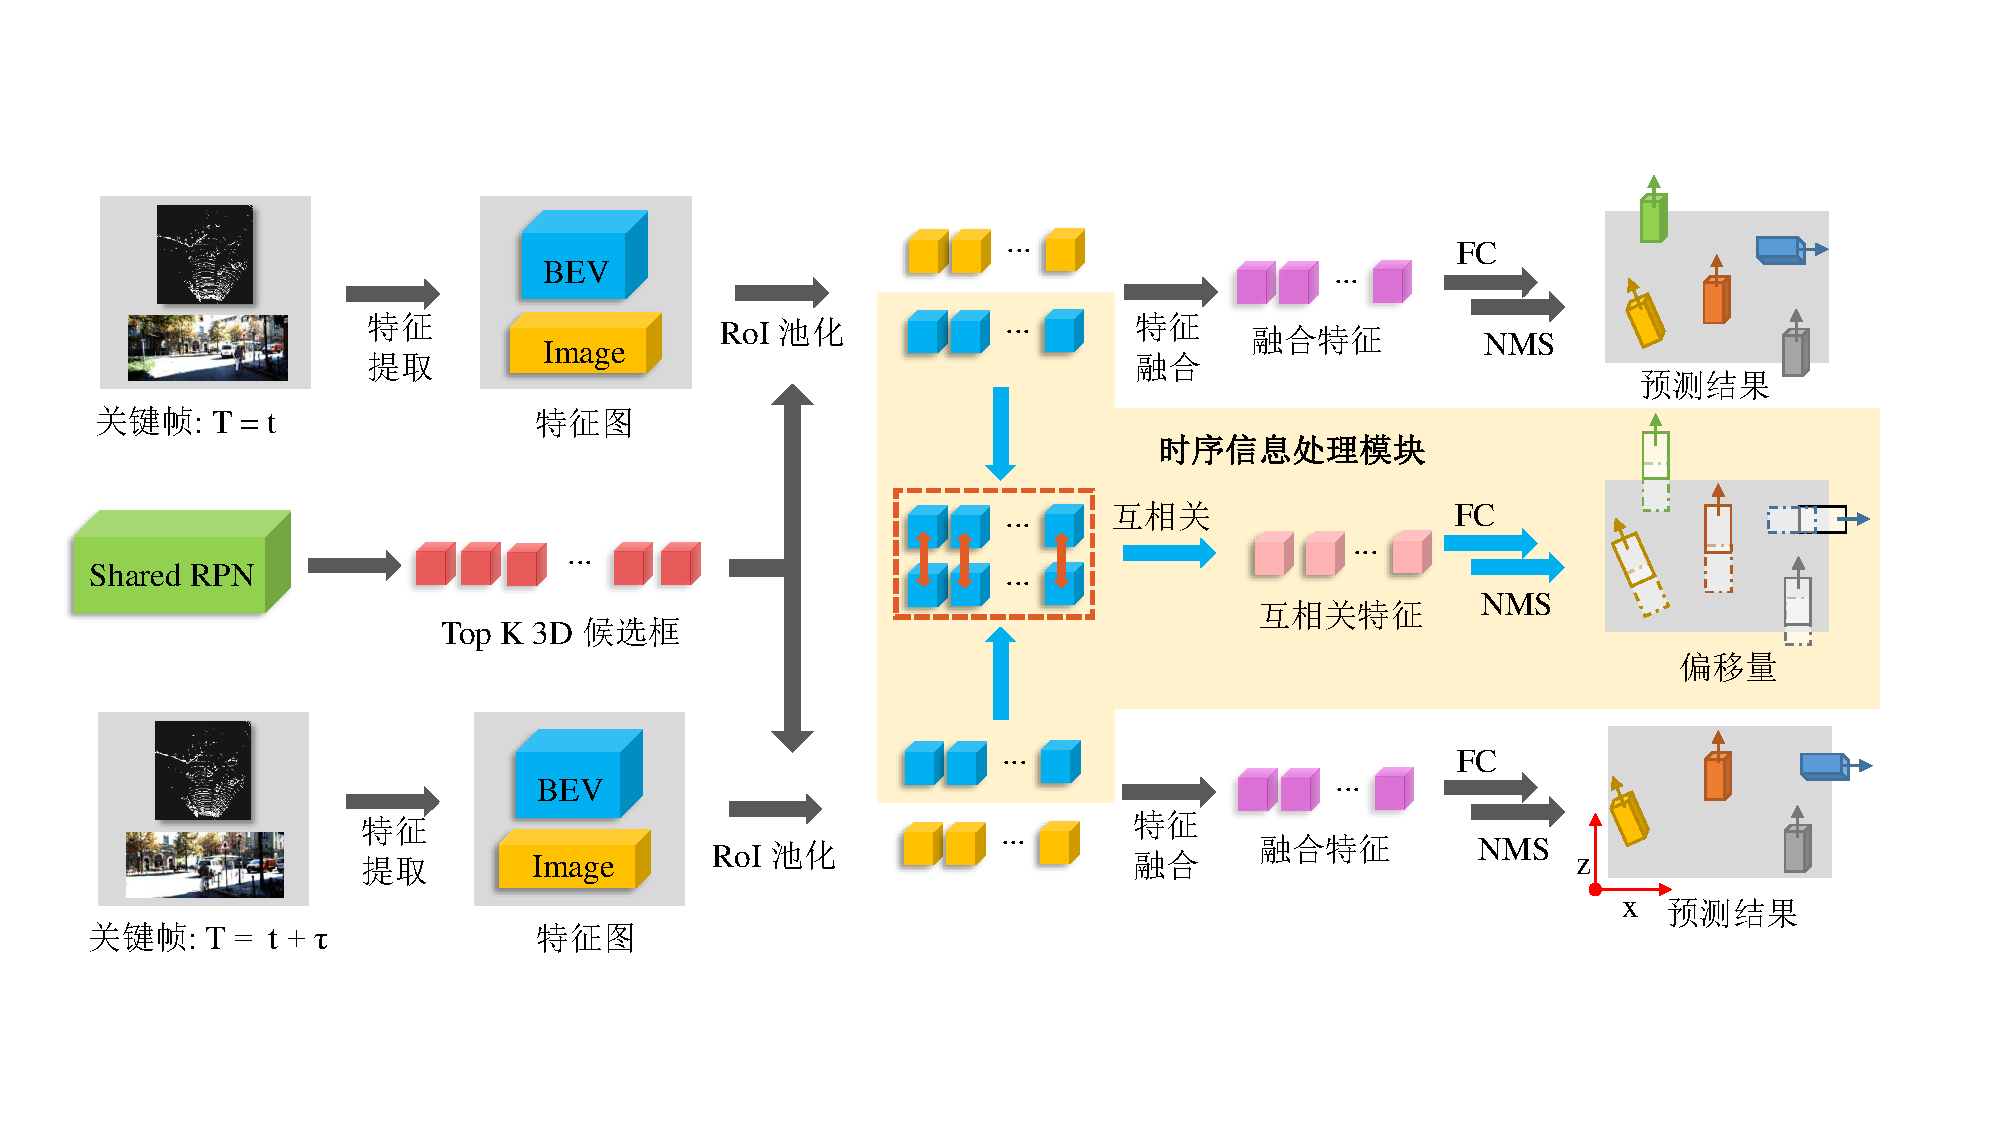
\includegraphics[trim={1.1cm, 2.5cm, 1.5cm, 2.5cm}, clip, width=\textwidth]{imgs/structure_final.pdf}
	\end{center}
	\vspace{-0.8cm}
	\caption{DODT 框架结构,FC表示全连接层,NMS是非极大值抑制过程。}
	\label{fig:dodt}
	%\vspace{-0.3cm}
\end{figure}


DODT网络是双路结构,其结构如\figurename \, \ref{fig:dodt} 所示。DODT由四个小模块组成:三维物体检测模块、Shared RPN模块、时序信息处理模块以及运动插值模块。三维物体检测模块有两个分支,分别负责检测两相邻关键帧中的物体,两分支的网络结构相同,并且共享参数。检测模块的网络结构是基于AVOD\cite{ku2018joint}构建的,为二阶段物体检测框架的三维扩展,该模块的详细结构将在3.2节介绍。Shared RPN 模块负责生成二阶段物体检测中的候选框,与传统RPN不同的是,Shared RPN生成的3D候选框可以被两个三维检测分支共同使用,该模块将在3.3节详细介绍。时序处理模块为 \figurename \, \ref{fig:dodt} 的浅黄色区域,该模块通过对相邻关键帧的点云俯视图(Bird Eye View,BEV)特征匹配块进行相关(correlation) 操作提取帧间的时序信息,然后预测同一物体物体在两关键帧的位置位置偏移。3.4节将详细介绍时序处理模块的实现原理。运动插值模块主要是由独立于网络结构的运动插值算法构成,该算法使用三维物体检测模块对两关键帧的检测结果以及时序处理模块输出的位置偏移信息,将关键帧的检测结果传播到非关键帧,实现流数据的三维物体检测与追踪。该算法的详细流程将会在3.5节重点介绍。


\section{三维物体检测模块}
\label{3d_detection_module}

DODT框架的三维物体检测模块融合了点云与图像信息,预测自动驾驶场景中车辆的三维位姿信息。由于该检测模块是基于AVOD\cite{ku2018joint}网络,为二阶段物体检测模块,因此包含候选框提取网络。由于本框架的候选框提取网络与AVOD有所不同,因此将在下一节详细介绍。本节不展开介绍候选框提取环节。本节将依次介绍数据预处理、特征提取、RoI池化、特征融合以及最终的预测框生成等物体检测中的关键步骤。

\subsection{数据预处理}

DODT融合RGB图像数据以及激光雷达数据进行三维物体检测,因此每一帧数据都同时包含图像以及点云。RGB图像数据预处理比较简单,首先统一调整长宽到$1200 \times 360 $ px,然后在RGB通道上将去数据集的RGB平均值$[R_{mean},G_{mean},B_{mean}]$(本工作基于的KITTI下的物体追踪数据集,RGB平均值为[92.84,97.80,93.58])。RGB图像数据经过色彩均值归一化后就可以直接用于后续的特征提取操作了。

点云数据的预处理相对于图像要更为复杂,这是因为点云是稀疏的三维数据,需要经过额外的操作将其转换为网络能够处理的形式。本工作采用网格化的方法将点云数据编码成六通道的BEV特征图,特征图包含五个高度切片通道以及一个点云密度信息通道。我们首先将点云投影到相机平面,然后过滤落在图像尺寸之外的点以便让点云视野与图像视野相同【TODO】。对于截取得到的规则三维视野,我们首先使用0.1m分辨率的网格将XZ平面网格化。假设XZ平面尺寸为 $[-W,W] \times [0, L] m$,则网格化后的尺寸为$\frac{2W}{0.1} \times \frac{L}{0.1}$。对于高度Y方向,我们截取$[0,2.5] m$ 的区域,然后平均切片为五等份从而将整个点云体素化。而后,将每个体素格子中所有点高度的最大值作为该格子的值,从而将点云编码为BEV特征图。对于特征图的最后一个通道,我们使用高度切片前的每个格子内的点计算该格子的点云密度 $\rho = \min(1.0, \frac{\log(N+1)}{\log 16})$,其中$N$为格子内点的数目。该方法最先在MV3D\cite{chen2017multi}中使用,而后AVOD\cite{ku2018joint}也使用了相同的处理方式。

在自动驾驶场景中,车辆是不停运动的,因此流数据中每一帧数据的参考系也不同。为了更好的关联帧与帧之间的时序信息,除了对每一帧数据进行预处理外,还需将不同帧的数据校准到同一坐标系。DODT为双路结构,同时处理相邻两帧关键帧数据并关联帧间信息。因此,为了统一两帧数据的坐标系,我们将后一帧关键帧数据校准到前一帧数据的坐标系中。由于图像数据没有准确的三维坐标信息,我们只校准点云数据。点云数据的校准需要用到激光雷达的位姿信息,这些数据KITTI数据集有提供。

\subsection{特征提取}

\begin{figure}
	%\vspace{-0.5cm}
	\centering
	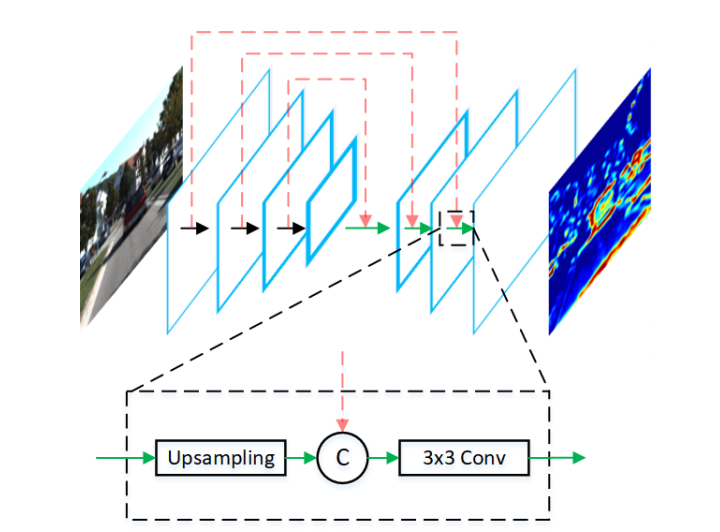
\includegraphics[width=0.8\textwidth]{imgs/feature-extractor.png}
	%\vspace{-0.3cm}
	\caption{特征提取网络结构。}
	\label{fig:feature_extractor}
	%\vspace{-1.5cm}
\end{figure}


DODT检测模块有两个单独的特征提取网络,分别用于图像特征提取以及点云特征提取。这两个网络的结构类似,只是输入的尺寸不一样。特征提取网络采用的编码器-解码器(Encoder-Decoder)结构,包含了编码器和解码器两部分,如\figurename \ref{fig:feature_extractor} 所示。编码器基于VGG-16网络改造的,首先将网络的通道数减半,并在conv-4层截断。编码器输入尺寸为 $M \times N \times D$ 的图像数据或是点云BEV特征图,然后输出尺寸为 $\frac{M}{8} \times \frac{N}{8} \times D^*$ 的特征$F$。特征$F$能够表达高层次的语意信息,并且尺寸比输入小了八倍。KITTI数据集中行人在BEV视角平均大小为$0.8 \times 0.6$ 米,在BEV特征图上就是$8 \times 6$ 的像素区域(分辨率为0.1m)。在编码器八倍下采样后,行人在输出特征$F$中占据不到一个像素,这还是在不考虑卷积过程中感受野的放大所造成小物体占比缩小的情况。受特征金字塔网络(Feature Pyramid Network)的启发,AVOD设计了一个自底向上的解码器,解码器可以在几乎不增加运行时间的基础上,将特征$F$上采样到输入的尺寸大小。解码器将编码器的输出作为输入,然后生成尺寸为$M \times N \times D$ 的特征图。解码器的上采样是通过反卷积算子实现的,为了更好的补回编码器中下采样造成的细节损失,解码器每一层的输入还额外包含编码器对应层的特征,然后通过一个$3 \times 3$的卷积操作融合。最终的特征图在保留了对高层语意的表征能力下,还能有与输入相同的尺寸,这在一定程度上避免了小物体特征丢失的问题。

\subsection{特征融合}

\begin{figure}[t]
	\centering
	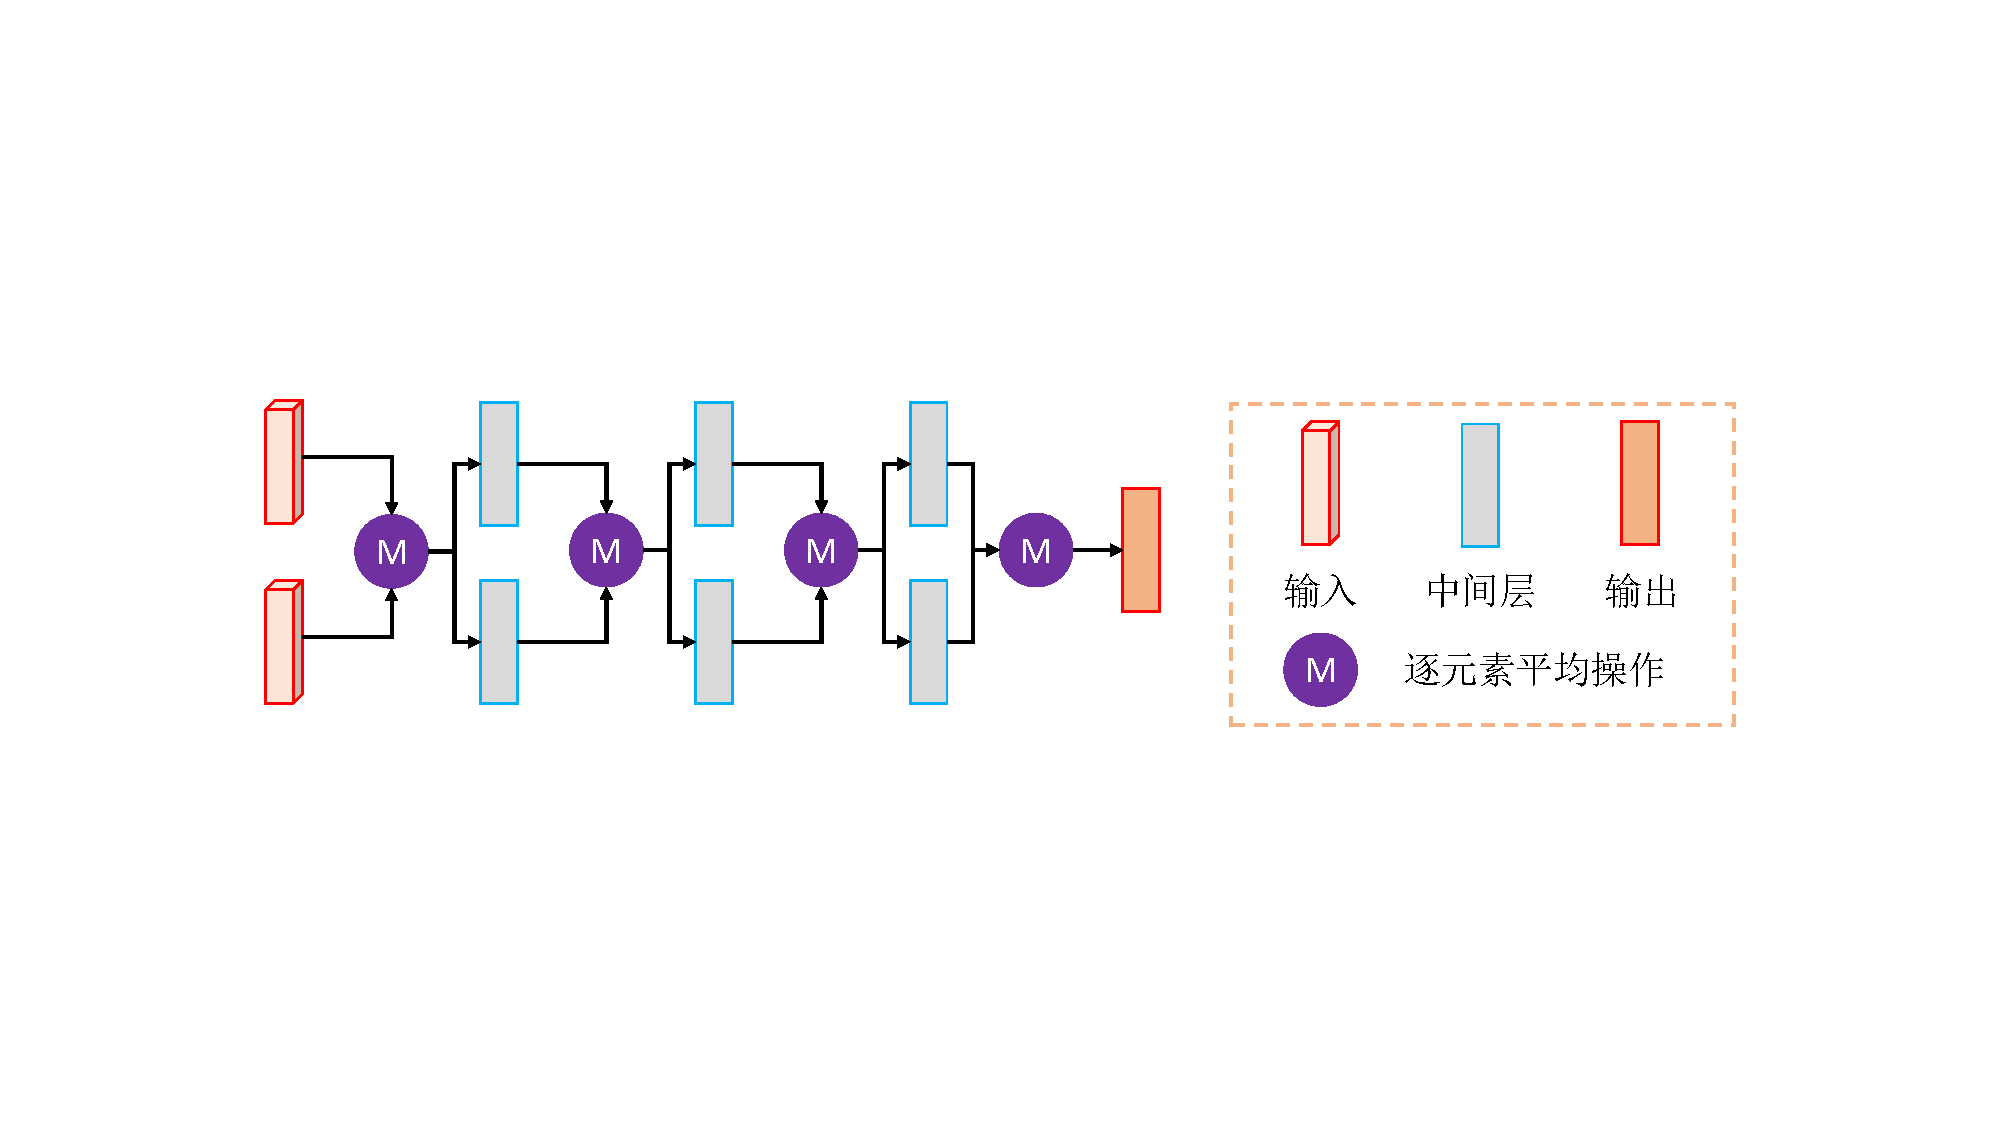
\includegraphics[trim={4cm, 6cm, 4cm, 6cm}, clip, width=\textwidth]{imgs/fusion-network.pdf}
	\caption{深度融合网络(deep fusion)结构,输入为点云BEV特征$f_{img}$以及图像特征$f_{pc}$。}
	\label{fig:fusion_network}
\end{figure}


在特征提取阶段我们分别得到了图像的特征$F_{img}$以及点云的特征$F_{pc}$,接下来就是将这两种特征融合以得到更丰富的视觉特征。DODT的特征融合也是借鉴了AVOD的方式,在候选框层面上进行融合。给定一个3D候选框由(Shared RPN生成),将其投影到$F_{img}$以及$F_{pc}$上,截取相应的部分就能得到对应的候选区域特征$f_{img}$ 以及$f_{pc}$。之后$f_{img}$ 和 $f_{pc}$ 将会通过$7 \times 7$的ROI池化操作生成相同尺寸的特征向量,之后两特征向量通过一个融合网络生成最终的候选区域特征向量$F_{fusion}$。融合网络结构如\figurename \ref{fig:fusion_network} 所示,该网络结构最先由MV3D提出,叫做深度融合网络。对于有$L$层的网络,深度融合网络按如下方式融合特征:
\begin{equation}
	\begin{aligned}
		& F_0 = F_{img} \oplus F_{pc}\\
		& F_l = H^{img}_l(F_{l-1}) \oplus H^{pc}_l(F_{l-1})\\
		& \forall l = 1, ..., L
	\end{aligned}
\label{con:deep_fusion}
\end{equation}
其中,$\{H_l, l=1,...,L\}$是特征转移函数(由神经网络拟合),$\oplus$为某种融合操作(例如拼接、求和等,DODT使用的是平均)。深度融合网络可以让两种特征能在更深层次、更高的语意层面进行融合,从而取得更好的融合效果。

\subsection{预测框生成}

\begin{figure}[t]
	\centering
	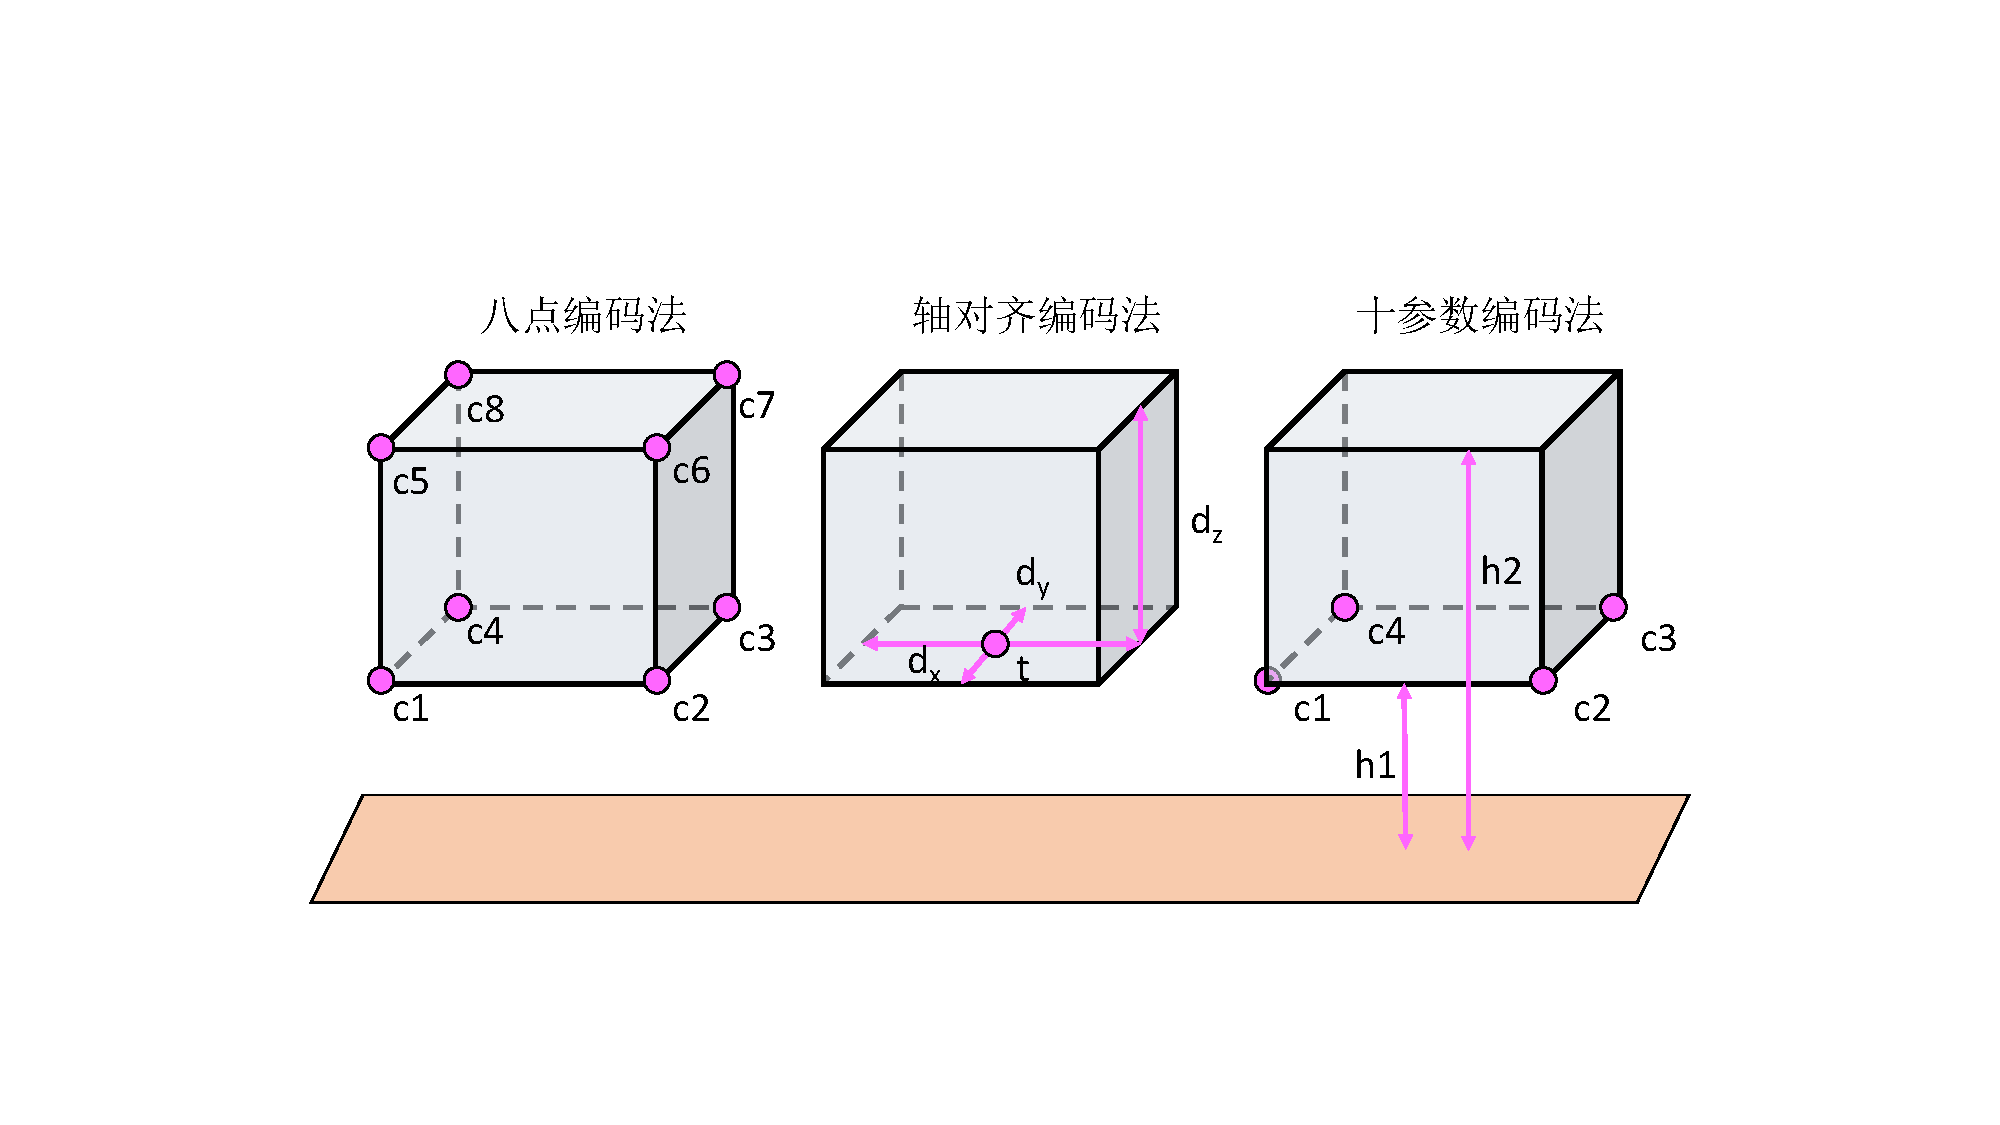
\includegraphics[trim={5cm, 3.5cm, 5cm, 4cm}, clip,width=\textwidth]{imgs/box-encoding.pdf}
	\caption{三种三维框编码方式。}
	\label{fig:box_encoding}
\end{figure}


特征融合之后,融合的特征图将会输入到两个不同任务分支,分别为检测分支和回归分支, 这两个分支都是由三层2048个神经元组成的全连接层。检测分支负责预测目标的类别,使用交叉熵计算损失值;而回归分支负责预测候选框与真实物体框的差值,使用$Smooth \, L1$ 函数计算损失值。在回归损失中,只有当候选框与真实框在BEV视角的 2D IoU 大于 0.65 才会被计算。之后, DODT使用NMS算法去除重叠的框,阈值设置为 0.01。

在框回归中,对三维框的编码有很多种方式,其中比较常见的有八点编码法和轴对齐(Axis Aligned) 编码法,如\figurename \ref{fig:box_encoding} 所示。八点编码法直接编码八个顶点的坐标,这种方式没有考虑三维框自身的几何约束,有一定的冗余性。而轴对齐编码限制了三维框要和坐标轴对齐,这是在RPN阶段使用的,并不适合最终的框编码。DODT使用了AVOD提出的10参数编码法,如\figurename \ref{fig:box_encoding}最右侧所示,分别编码底部四点坐标以及底面与顶面和地面的距离,一共有十个参数,因此框回归的目标为 $(\Delta_{x1}, ...,\Delta_{y1}, \Delta_{y4}, \Delta_{h1}, \Delta_{h2})$。这种编码方式考虑到了三维框顶面四点和底面四点是对齐的,而原来的过参数化的八点法需要编码成24维向量。

在MV3D中,作者默认三维预测框的朝向为长边方向,可是这种确定朝向的方法是有问题的。首先并不是所有目标都适用于这种确定朝向的方法,比如行人;其次,长边有两个可取的方向,它们相差 $\pm \pi$。AVOD中,作者通过预测转向向量 $(x_{\theta},y_{\theta}) = (\cos(\theta), \sin(\theta))$来解决这个问题。这种方式可以将每个转向角$\theta \in [-\pi, \pi]$都映射到唯一的转向向量。转向向量的预测也是包含在回归分支中。另外,转向向量可以用来解决十参数编码法中预测框与真实框底部四点的对应关系。底部四点的对应有四种,只使用十参数编码时只能通过最近匹配法,有了转向向量之后,转向向量的值可以作为额外的匹配手段。


\section{Shared RPN模块}
\label{shared_rpn}

\begin{figure}
	%\vspace{-0.5cm}
	\centering
	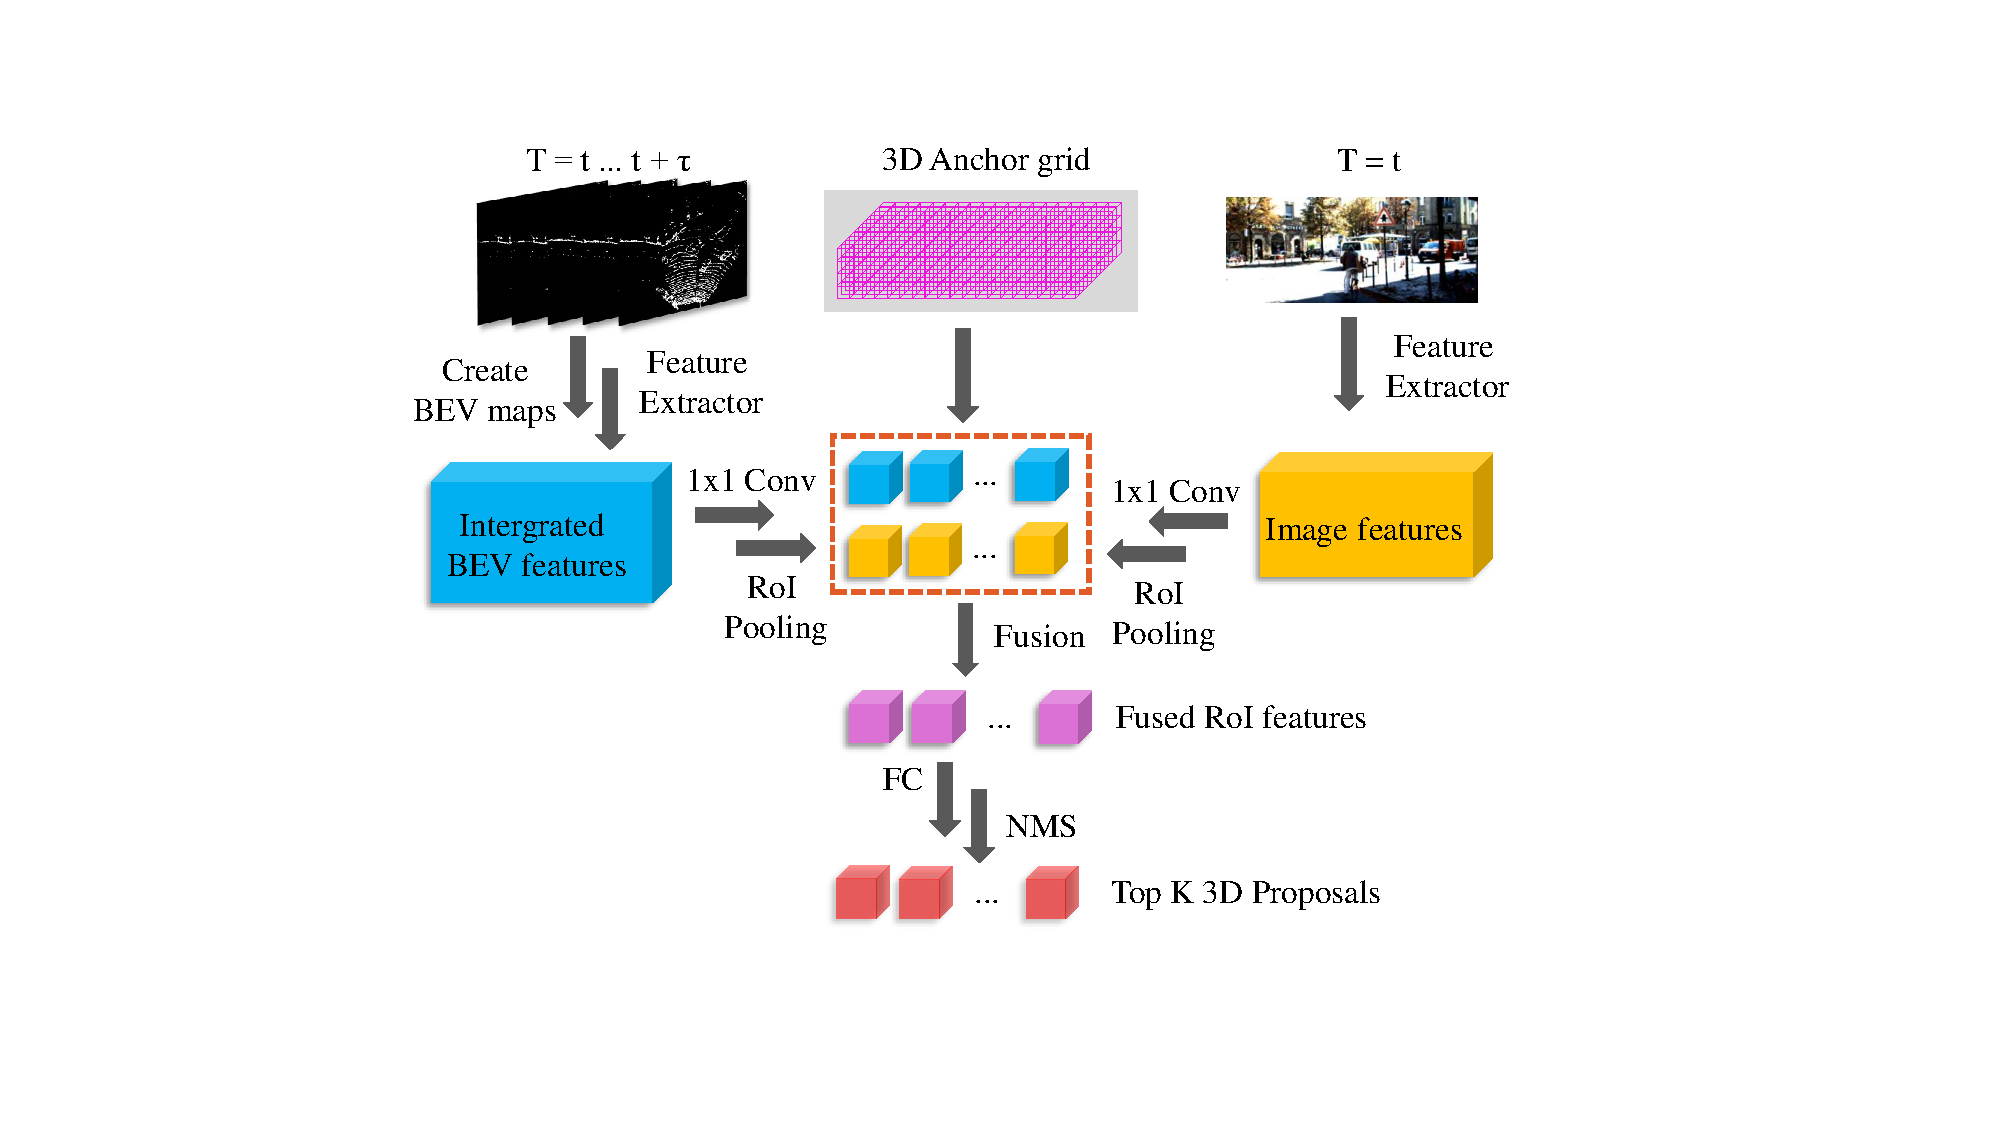
\includegraphics[trim={7cm, 3cm, 8cm, 2cm}, clip,width=0.9\textwidth]{imgs/rpn_final.pdf}
	%\vspace{-0.3cm}
	\caption{Shared RPN 模块。}
	\label{fig:shared_rpn}
	%\vspace{-1.5cm}
\end{figure}


DODT 的 \textit{Shared RPN} 模块是以 AVOD 的 RPN 为基础改造的,其结构如\figurename \ref{fig:shared_rpn}所示。DODT有两个检测分支,正常来说需要两个单独的RPN网络生成各自的候选框。但由于DODT处理的是流数据,两分支的关键帧输入有很大的关联性,因为关键帧的特征变化在时间维度上是连续的。受此启发,我们将两分支的RPN合并成一个\textit{Shared RPN},该RPN能够生成供两分支同时使用的3D候选框。和检测模块一样,\textit{Shared RPN}也融合了点云特征与图像特征来预测3D候选框。图像数据的处理和检测模块一样,由于相邻关键帧中图像数据的变化微乎其微,因此我们只使用前一帧关键帧图像数据提取RGB特征,特征提取过程和检测模块一样(可以直接使用检测模块处理好的图像特征)。对于点云特征提取,\textit{Shared RPN}不像检测模块一样只使用一帧点云数据,而是联合了两关键帧以及关键帧之间的点云数据。这是因为点云数据是稀疏的,单帧点云数据不能很好的捕获物体在三维空间的位姿信息,特别是对于远处的物体。但如果将连续时间片段的点云数据联合起来,这在一定层度上是能够增强物体特征的。考虑到在实际驾驶场景中LIDAR本身也在不停地运动,造成每帧点云的参考系不一样,直接叠加点云数据效果必然很糟糕,因此需要把这些点云数据校准到同一坐标系上。点云的校准需要用到LIDAR在不同时刻的位姿信息,这些可以在IMU数据中得到。将连续时间片段的点云数据校准到同一坐标系后,使用和检测分支一样的方式构建BEV特征图,然后用相同的特征提取网络提取点云特征。由于点云的稀疏性以及使用体素化的点云编码方法,点云数据的联合并不会带来额外的计算负担,但却可以有效的增强点云特征。

\begin{figure}[t]
	\begin{center}
		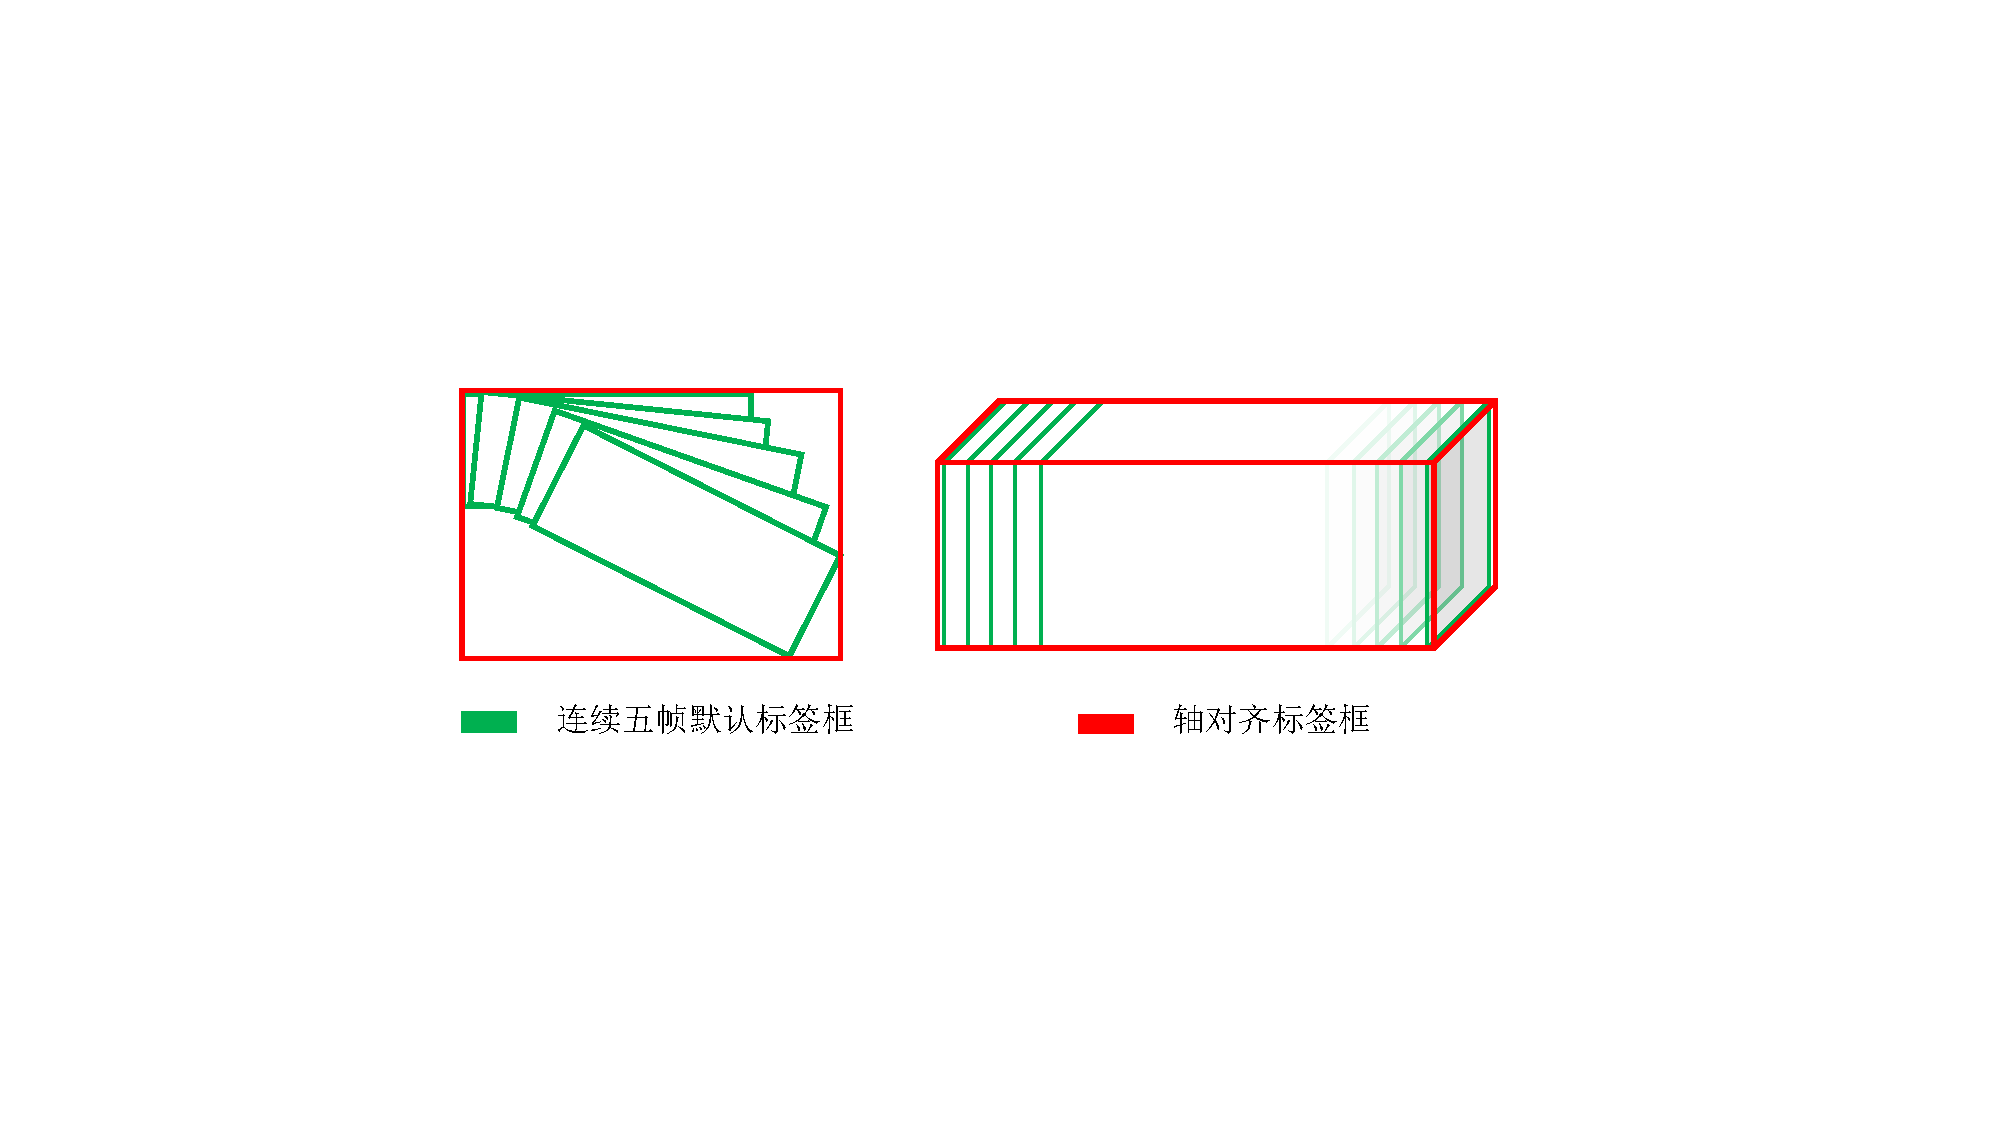
\includegraphics[trim={6cm, 6cm, 8cm, 6cm}, clip, width=0.8\textwidth]{imgs/axis-aligned-boxes.pdf}
	\end{center}
	\vspace{-0.8cm}
	\caption{\textcolor{green}{绿色} 框是五帧中目标的标签框,\textcolor{red}{红色}框是为训练\textit{Shared RPN} 而新生成的共享候选框标签。}
	\label{fig:integrated_boxes}
\end{figure}


需要额外注意的是,由于物体在不断运动,因此联合的点云数据标签需要重新计算。假设一目标在联合的五帧点云数据中都有出现,那么新的标签应该囊括该目标在这段时间内的运动轨迹。如\figurename \ref{fig:integrated_boxes}所示,我们重新计算了适合\textit{Shared RPN}训练的新的候选框标签。新的候选框标签可以同样也是轴对齐的,虽然相比于之前的候选框标签略有增大,但这能够保证覆盖物体在所有融合帧中的运动轨迹,从而使其适合训练生成供两检测分支使用的3D 候选框。

拿到点云特征与图像特征之后,需要经过和检测模块一样的流程融合两个视角的特征。特征的融合是在锚点框层面的,DODT锚点框的尺寸是通过对KITTI目标检测数据集的标签进行聚类得到。通过将3D锚点框投影到两特征图上,然后截取相应的区域再进行ROI池化得到特征块,特征块再通过深度融合网络得到最终的融合特征。\textit{Shared RPN}的特征融合过程和检测模块的基本类似,但是前者的图像特征图与点云特征图在进行ROI池化前,都经过了一个 $1 \times 1$ 的卷积将特征通道数降为1。这是因为在某些场景下,锚点框可以多达100K个,直接从全通道的特征图上去截取特征块会给GPU带来巨大的存储负担。例如,提取100K个通道为256的$7 \times 7$特征块需要将近5GB存储($100000 \times 7 \times 7 \times 256 \times 4 \text{ bytes}$,假设以32位浮点数存储)。此外,处理如此大通道的特征也会让RPN耗费巨大的计算资源。因此\textit{Shared RPN}通过一个$1 \times 1$的卷积操作进行数据降维,能有效减低网络参数量,提升运行效率。而在检测模块中,为追求更高的检测精度,仍维持原来的通道数。

融合网络生成的融合特征最终被用来预测候选框的尺寸和类别。和检测模块类似,有候选框分类和回归两个分支。分类分支是由两层256个神经元的全连接层组成,用来预测候选框是目标区域还是背景区域,为二元分类任务。回归分支同样也是由两层256个神经元的全连接层组成,回归出预测候选框与真实候选框之间的偏差 $(\Delta t_x,  \Delta t_y, \Delta t_z, \Delta d_x, \Delta d_y, \Delta d_z)$。候选框的编码方式如\figurename \ref{fig:box_encoding}中间所示,包含底部中心点坐标$(t_x, t_y, t_z)$ 以及长宽高$(d_x, d_y, d_z)$。这是因为候选框都是轴对齐的,所有只需要六个参数就能够编码一个三维框。和检测模块一样,分类分支以交叉熵作为损失函数,而回归分支则使用$Smooth \, L1$ 作为损失函数。当锚点框与真实框在BEV视角的2D IOU 值小于0.3时将被视为背景类,而大于0.5时被视为目标类,回归损失值的计算不将背景类的损失值。最后,2D NMS算法会被用于筛除重叠的候选框。网络训练阶段NMS算法的阈值是0.8,保留最好的1024个候选框,而在预测阶段则只保留最好的300个候选框。

\section{时序信息处理模块}
\label{temporal_module}

时序信息处理模块输入相邻关键帧的点云BEV特征,然后预测两帧中相同物体的位移,其结构如\figurename \, \ref{fig:dodt}黄色区域所示。关键帧$t$以及$t+\tau$的特征图经过ROI池化后分别得到对应的RGB和点云特征块$(F^t_{img}, F^t_{pc})$和$(F^{t+\tau}_{img}, F^{t+\tau}_{pc})$,时序模块只使用点云特征块$F^t_{pc}$和$F^{t+\tau}_{pc}$预测偏移量。这是因为DODT只考虑BEV视角的偏移量,因为在自动驾驶场景中,车辆行驶区域基本可以视为二维平面,高度变化不会太大,故只预测车辆在BEV视角的偏移量就能够很好的捕获车辆的运动信息。给定两相邻关键帧的点云BEV特征块集合$F^t_{pc}$和$F^{t+\tau}_{pc}$,时序处理模块首先构造一个特征块对集合$P = \{(f^t_i, f^{t+\tau}_i), i \in \{0, 1, ..., N\}\}$,其中$f^t_i$和$f^{t+\tau}_i$分别是$F^t_{pc}$和$F^{t+\tau}_{pc}$的第$i$个特征块,$N$是3D候选框的总数,也是两关键帧特征块的总数。由于两检测分支使用相同的3D候选框(由 \textit{Shared RPN}生成),因此两特征块集合$F^t_{pc}$和$F^{t+\tau}_{pc}$的元素是相互对应的,因此$P$很容易生成。

构建好特征块对集合$P$之后,模块对$P$的每一个元素$(f^t_i, f^{t+\tau}_i)$使用相关操作,如公式\ref{con:correlation}所示,其中$p,q \in [-d, d]$ 是相关计算的偏移量,$d$是窗口大小,$j,k$是窗口中心点坐标。相关特征的输出$C \in \mathbb{R}^{h \times w \times (2d+1) \times (2d+1)}$,其中 $h,w$是特征块的宽和高。由于总共有$N$对特征块对,最终会有$N$个相关特征输出。这些特征会输入全连接层进行后续的分类与回归任务。
\begin{equation}
C^{t,t+\tau}(j,k,p,q) = \left \langle f^t_i(j,k), f^{t+\tau}_i(j+p,k+q) \right \rangle
\label{con:correlation}
\end{equation}

时序信息处理模块有两个输出分支,一个是分类分支,预测该物体是否同时存在在两帧关键帧中;另一个分支是回归分支,预测该物体在两关键帧中的相对位移(BEV视角)。分类分支由两层256个神经单元的全连接层组成,它的输出是一个概率值$p_{co}$,表示两帧中都存在该物体的概率(Object co-occurrence probability), 当物体同时存在两帧中时,$p_{co} = 1$,否则 $p_{co} = 0$。$p_{co}$的值可以用来判断物体轨迹的开始或终止,以及是否存在漏检现象。$p_{co}$的计算主要是为后续的运动插值模块的正确运行提供额外的保障,这部分内容将在运动插值模块详细介绍。

回归分支的任务比较简单,它也是由两层256个神经单元的全连接层组成,负责预测同一个物体在两帧的相对位移。假设$d^t = (x^t, z^t,\theta^t)$ 为第$t$帧中一物体的X轴和Z轴(深度方向)坐标以及转向角,相同的,$d^{t+\tau} = (x^{t+\tau}, z^{t+\tau},\theta^{t+\tau})$为$t+\tau$帧中该物体相应的数据,则回归分支负责预测$d^t$与$d^{t+\tau}$的归一化偏差$\delta^{t,t+\tau}$,如公式\ref{con:correlation_offsets}所示,
\begin{equation}
\delta^{t, t+\tau} = (\delta_x^{t,t+\tau}, \delta_z^{t,t+\tau}, \delta_{\theta}^{t,t+\tau}) = \\
\begin{cases}
(\frac{x^{t+\tau} - x^{t}}{w^t}, \frac{z^{t+\tau} - z^{t}}{l^t}, \frac{\theta^{t+\tau} - \theta^{t}}{\theta^t}) & p_{co} = 1.0 \\
(0.0,0.0, 0.0) &  otherwise
\end{cases}
\label{con:correlation_offsets}
\end{equation}
其中$w^t$和$l^t$分别是物体在第$t$帧的宽和长。当$p_{co}$为1.0时,意味着该物体同时存在两帧中,故可按公式正常计算相对偏差;而当$p_{co} = 0$时,意味着该物体只存在某一帧中,这时$\delta^{t,t+\tau}$的值将无法计算,我们将其置为0。在网络训练中,分类分支的损失函数是交叉熵,而回归分支的损失为$Smooth \, L1$。

\section{运动插值模块}
\label{interpolation}

\begin{figure}[t]
	\begin{center}
		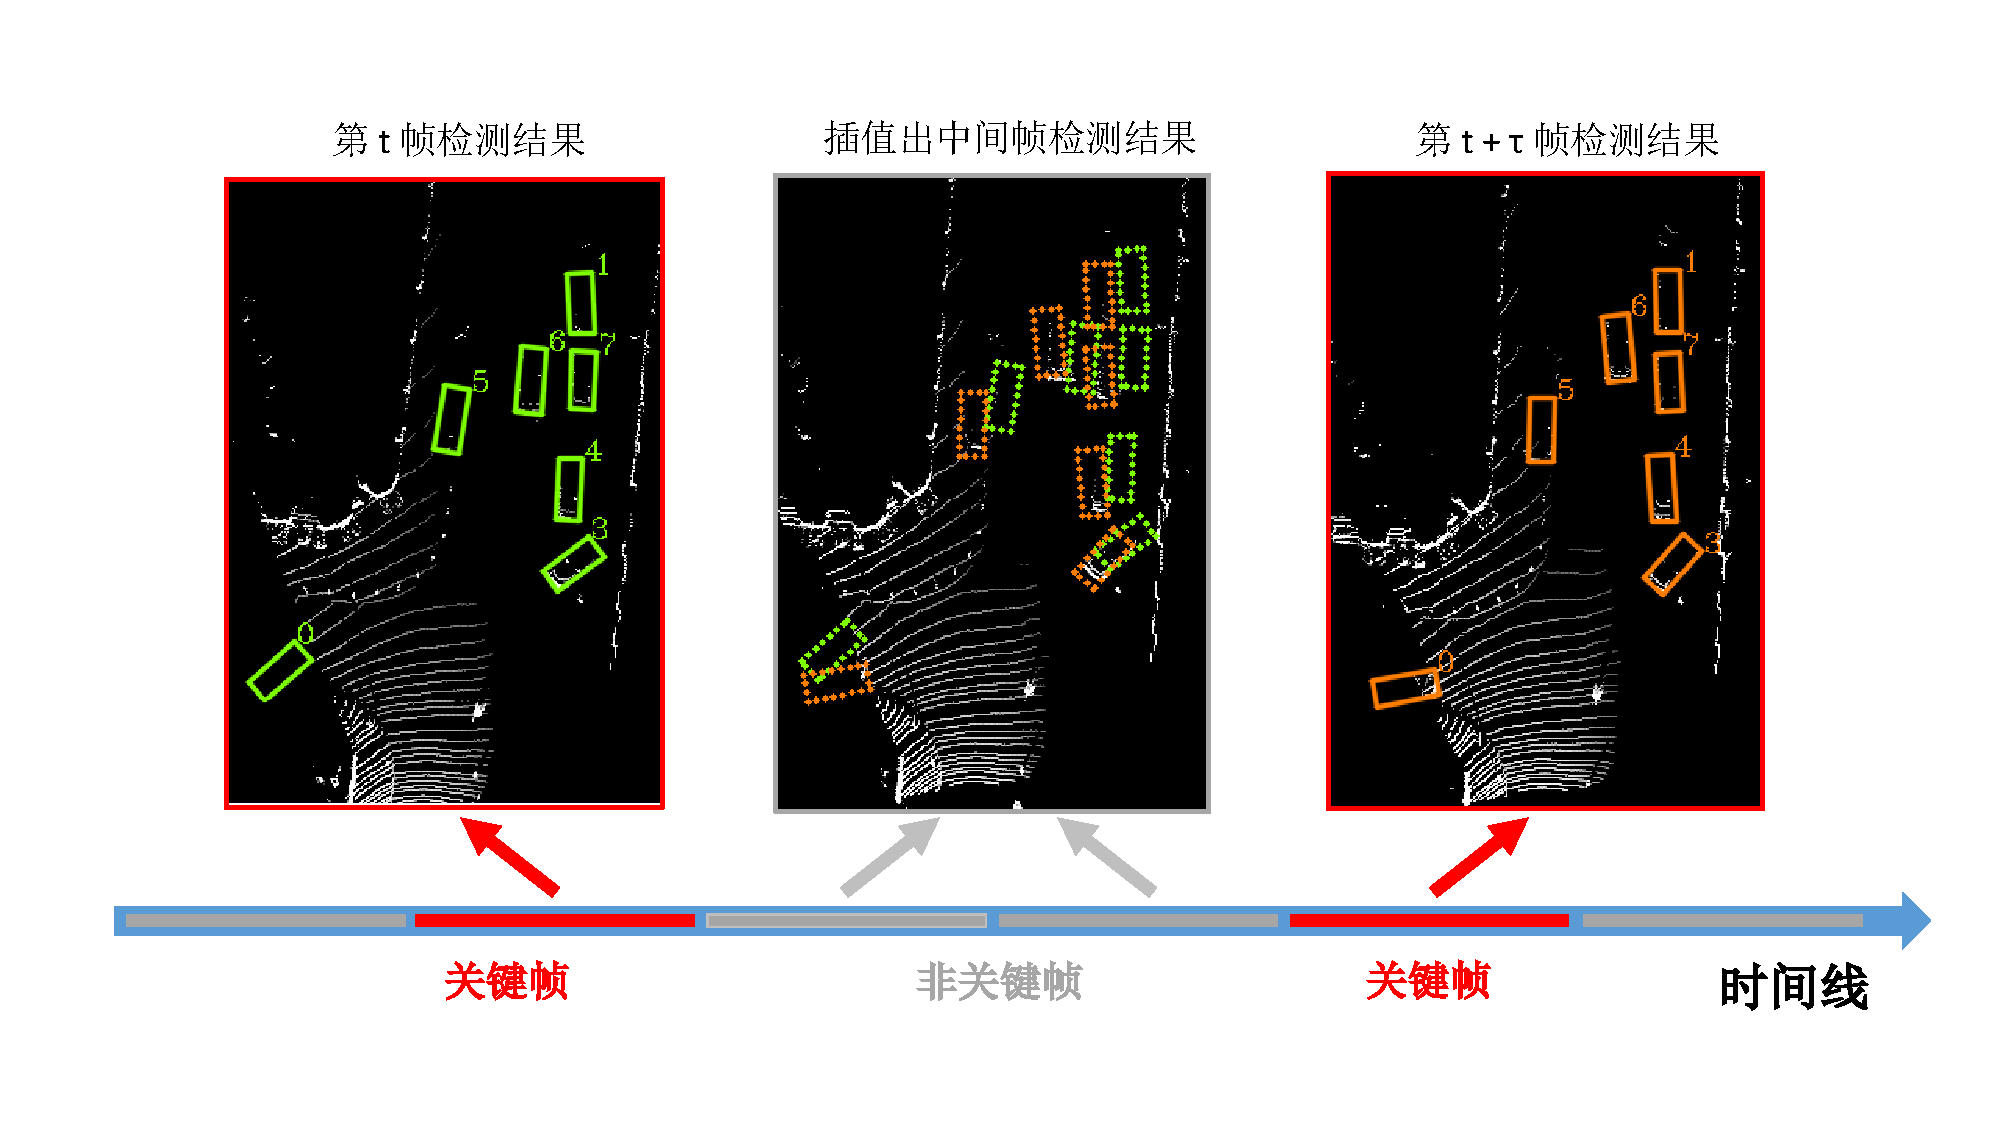
\includegraphics[trim={1.1cm, 1cm, 1.5cm, 1cm}, clip, width=\textwidth]{imgs/timeline_interpolation.pdf}
	\end{center}
	\vspace{-0.8cm}
	\caption{运动插值模块实现的是将关键帧检测结果传播到非关键帧。}
	\label{fig:timeline_interpolation}
\end{figure}


运动插值模块的任务主要是将两目标检测模块的输出与时序信息处理模块的输出整合,在时序信息的引导下,将关键帧的物体检测结果传播到非关键帧,如图\ref{fig:timeline_interpolation}所示。运动插值模块主要由一个基于运动模型的插值算法(Motion based Interpolation Algorithm,MoI)组成,其流程如算法 \ref{alg:interpolation} 所示。MoI算法的输入为第$t$帧以及$t+\tau$帧的三维物体检测结果$D^t$和$D^{t+\tau}$,以及这两帧中各物体的相对偏移$\Delta^{t,t+\tau}$。输出为$t$到$t+\tau$帧的所有目标检测结果。当$t$帧与$t+\tau$帧检测的目标个数相同时,$D^t,D^{t+\tau}$以及$\Delta^{t,t+\tau}$元素个数相同;当有目标不同时存在于$t$帧与$t+\tau$帧时,$D^t$与$D^{t+\tau}$的元素不相等,而$\Delta^{t,t+\tau}$元素个数为$D^t$与$D^{t+\tau}$的最大值,只是不同时存在前后两帧赶关键帧的目标偏移量为0。

\begin{algorithm}[!h]
	\caption{基于运动模型的插值算法(MoI Algorithm)}
	\label{alg:interpolation}
	\textbf{输入: } $D^t= [d^t_0, d^t_1, ..., d^t_{N_t}], D^{t+\tau}= [d^{t+\tau}_0, d^{t+\tau}_1, ..., d^{t+\tau}_{N_{t+\tau}}],$
	$\Delta^{t, t+\tau}=[\delta^{t, t+\tau}_0, \delta^{t, t+\tau}_1, ..., \delta^{t, t+\tau}_{N_{max}}], N_{max} = \max\{N_t, N_{t+\tau}\}$\\
	\textbf{输出: } $D = [D^t, D^{t+1}, ..., D^{t+\tau}]$\\
	\textbf{初始化:} $D_{temp} = D^{t+\tau}, D, p_{co}^{max} = 0.5$ \\
	\For{$d^t_i \emph{ in } D^t$}{
		$\Delta d^{t, t+ \tau}_{i} = (d^t_{i, w} \cdot \delta^{t, t+\tau}_{i,x}, 0, d^t_{i, l} \cdot \delta^{t, t+\tau}_{i,z}, 0, 0, d^t_{i, ry} \cdot \delta^{t, t+\tau}_{i,ry})$
		$d' = getMatched(d^t_i+\Delta d^{t, t+ \tau}_{i}, D_{temp})$\\
		\If{$d'$ 存在}{
			$d^{t+1}_i,..., d^{t+\tau-1}_i = Interpolate(d^t_i, d')$\\
			将 $d'$ 从 $D_{temp}$ 中移除
		}
		\ElseIf{$p_{co}^i \geq p_{co}^{max}$}{
			$d^{t+1}_i,..., d^{t+\tau}_i = Interpolate(d^t_i, d^t_i + \Delta d^{t, t+ \tau}_{i})$
		}
		\Else{使用运动模型生成 $(d^{t+1}_i,..., d^{t+\tau-1}_i)$}
	}
	\If{$D_{temp}$ 非空}{
		\For{$d^{t+\tau}_j \emph{ in } D_{temp}$}{
			\If{$p_{co}^j \geq p_{co}^{max}$}{
				$d^{t}_j,..., d^{t+\tau-1}_j = Interpolate(d^{t+\tau}_j - \Delta d^{t, t+ \tau}_{j}, d^{t+\tau}_j)$
			}
			\Else{
				使用运动模型生成 $(d^{t+1}_j,..., d^{t+\tau-1}_j)$
			}
		}
	}
\end{algorithm}

MoI算法的主要思想是对于两帧中都存在的目标,使用线性插值算法生成中间帧的结果;对于只存在某一帧的目标,则使用基于时序信息的运动模型生成中间帧结果。具体流程如下:(1)对于$D^t$中的每一个预测框$d^t_i$,首先让其加上对应的偏移量$\Delta d_i^{t,t+\tau}$(该偏移量由 $\delta_i^{t,t+\tau}$ 解码得到),得到预测的运动后的物体框$d^t_i + \Delta d_i^{t,t+\tau}$。然后使用 \textit{getMatched} 匹配函数去$D_{temp}$中找到匹配度最高的候选框$d'$。\textit{getMatched}函数简单的计算$d^t_i + \Delta d_i^{t,t+\tau}$ 与$D_{temp}$中所有框的3D IOU值,然后在高于某一阈值(具体实现时为0.5)的IOU中筛选出最大者,然后返回其对应的预测框$d'$。(2)如果匹配成功,即$d'$存在,即证明该目标在两帧中同时存在,然后算法使用线性插值生成$t+1$到$t+\tau-1$帧预测框结果,同时将$d'$从$D_{temp}$中移除,防止后续再次被匹配。(3)对于匹配失败的情况,有两种可能的原因,发生漏检以及轨迹终止。这两种情况的判断可以通过时序信息处理模块的输出$p_{co}$,如果$p_{co}^i \geq p_{co}^{max}$,则表明该目标很大概率在$t+\tau$中存在,只是由于检测模型漏检了。这种情况下可通过偏移量信息计算出下一帧对应的物体框为$d^t_i + \Delta d^{t, t+ \tau}_{i}$,之后通过线性插值算法就能够生成中间帧的结果。如果$p_{co}^i < p_{co}^{max}$, 则表明轨迹已经终止,这种情况算法会根据目标的历史运动信息进行适当的轨迹扩展,下一段将重点介绍该过程。(4)循环完$D^t$中元素后,有可能$D_{temp}$中还存在预测框没有被匹配。这时也同样会出现两种情况,一种是前一帧中发生了漏检,另外就是该目标刚刚出现,这可以通过$p_{co}$的值加以区分。对于漏检的情况,算法会根据偏移信息生成前一帧的预测框,然后再通过线性插值算法生成中间帧的结果;对于目标刚出现的情况,同样的算法使用运动模型进行轨迹扩展。

运动模型的使用是基于假设“物体的速度在短时间内是不变的,与相机自身的运动无关”开展的。在物体运动时,模型会根据物体的历史状态以及运动增量来计算物体在下一时刻的状态。具体而言,模型记录着每条轨迹片段在BEV视角的全局速度$v = (v_x, v_z, v_{\theta})$,当下一帧有某个物体匹配到该轨迹时,该全局速度会被更新,更新方法如公式\ref{con:global_velocity}所示。其中$\alpha$衡量了轨迹下一时刻物体速度对轨迹全局速度的影响,在实际运行$\alpha = 0.8$。对于轨迹的终止,由于DODT只对关键帧进行检测,因此我们无法判断轨迹具体在$t$帧到$t+\tau$帧中的哪一帧终止。因此,对于在$t$帧存在而$t+\tau$中不存在的物体,我们统一将轨迹向后延伸3帧,延伸过程使用该轨迹的全局速度进行插值。如果在延伸过程中轨迹超出点云数据范围,则延伸会提前终止。同样,对于轨迹的起始,轨迹也会根据后续帧的信息进行前向延伸。这样做的好处是确保算法不会出现漏检的情况,因为在实际应用中,漏检往往要付出更高的代价。
\begin{equation}
\begin{aligned}
	& v_x = \alpha v_x + (1-\alpha)\frac{x^{t+\tau} - x^{t}}{\tau} = \alpha v_x + (1-\alpha)\frac{w^t \delta_x^{t,t+\tau}}{\tau}\\
	& v_z = \alpha v_z + (1-\alpha)\frac{z^{t+\tau} - z^{t}}{\tau} = \alpha v_z + (1-\alpha)\frac{l^t \delta_z^{t,t+\tau}}{\tau}\\
	& v_{\theta} = \alpha v_{\theta} + (1-\alpha)\frac{\theta^{t+\tau} - \theta^{t}}{\tau} = \alpha v_{\theta} + (1-\alpha)\frac{\theta^t \delta_{\theta}^{t,t+\tau}}{\tau}
\end{aligned}
\label{con:global_velocity}
\end{equation}

在具体实验过程中,我们发现物体运动方向的预测有时候在相邻关键帧会发生180度的转变,这使得在物体朝向插值过程中出现很大的偏差。为了解决该问题,我们使用了一个简单的朝向校准算法来维持轨迹朝向的连续性。对于一条轨迹$T^i_{match}$和下一帧中与该轨迹匹配的预测框$D^i_{match}$,如果这两者的朝向之差大于$\frac{\pi}{2}$($T^i_{match}$的朝向由该物体最后时刻的朝向决定),则将$D^i_{match}$的朝向角度加上$\pi$,即将$D^i_{match}$旋转180度,使其能够与轨迹的朝向基本保持一致,这样就不会出现物体朝向在相邻帧中突然变化很大的情况。

\section{多目标追踪}
\label{tracking_module}
在时序信息处理模块,我们已经把相邻关键帧间的中间帧的所有检测目标关联起来了,要关联所有帧的检测结果,只需要再将各关键帧关联就行了。有两种方案可以实现关键帧的关联,一种是在输入关键帧对上做文章,例如连续输入关键帧对为$(i, i+\tau), (i+\tau, i+2\tau), ...$ ,这样的话时序信息处理模块就可以将所有帧的检测结果关联;另一种方案是将关键帧结果单独进行数据关联,关联算法可以使用IOU匹配法或是卡尔曼滤波。当相邻关键帧的间隔$\tau$比较大时,第二种方法的匹配效果会下降,考虑到第一种方案的简便和高效性,DODT最终使用了第一种方案。由于本算法一次可以完成一个时间窗口内数据的多目标目标跟踪,因此为近似在线(Near Online)算法。

\section{本章总结}
\label{metho_conclusion}
本章重点介绍了本工作提出的流数据三维物体检测与跟踪框架DODT的结构与原理实现。首先3.1节介绍了DODT的整体框架,DODT由四个模块组成,分别是三维物体检测模块、Shared RPN模块、时序信息处理模块以及运动插值模块。这四个模块分别在3.2节、3.3节、3.4节以及3.5节分别介绍。特别的,本章最后还探讨了基于检测结果的多目标跟踪算法实现。本章内容为本文的重点,DODT集成了本工作的主要创新。下一章将介绍本工作如何通过具体实验,定性与定量的验证本框架的性能。

% 打印时插入必要的空白页
\ifprint
\newpage
\thispagestyle{empty}
\mbox{}

% 避免空白页影响页码编号
\clearpage
\setcounter{page}{10}
\fi